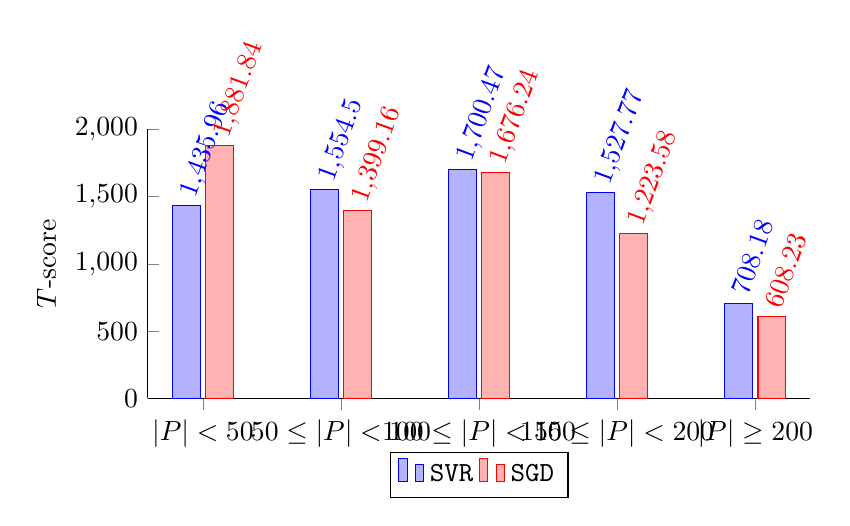
\begin{tikzpicture}
\begin{axis}[
	ybar,
	height=5cm,
	width=10cm,
	enlarge y limits=false,
	axis lines*=left,
	ymin=0,
	ymax=2000,
	legend style={at={(0.5,-0.2)},
		anchor=north,legend columns=-1},
		ylabel={$T$-score},
		symbolic x coords={50,100,150,200,201},
		xticklabels={
			$|P| < 50$,
			$50  \leq |P| < 100$,
			$100 \leq |P| < 150$,
			$150 \leq |P| < 200$,
			$|P| \geq 200$
		},
		xtick=data,
		nodes near coords,
		every node near coord/.append style={
			anchor=mid west,
			rotate=70
		}
	]
\addplot coordinates {
	(50,	1435.96)
	(100,	1554.50)
	(150,	1700.47)
	(200,	1527.77)
	(201,	708.18)
};
\addplot coordinates {
	(50, 	1881.84)
	(100,	1399.16)
	(150,	1676.24)
	(200,	1223.58)
	(201,	608.23)
};
\legend{\texttt{SVR},\texttt{SGD}}
\end{axis}
\end{tikzpicture}
